
\vspace{-1cm}
\chapter{Metodologia} \label{cap:metodologia}

\begin{comment}
Nesse capítulo será descrita a metodologia utilizada para o desenvolvimento deste projeto. Serão descritas as etapas do projeto e os principais fundamentos e tecnologias a serem empregados.

O trabalho será composto por seis etapas:

\begin{enumerate}
\item Projetar e montar a estrutura física.
\item Modelar o sistema.
\item Projetar e implementar o sistema de comunicação.
\item Projetar e construir o sistema embarcado.
\item Projetar e implementar o sistema de controle.
\item Idealizar e conduzir experimentos reais de teste de navegação.
\end{enumerate}

\noindent{\bf Etapa 1:} essa etapa será destinada ao projeto, aquisição e montagem da estrutura física do quadricóptero. A estrutura é composta basicamente por um chassi, quatro motores, quatro hélices e uma bateria. Deverão ser analisados os recursos disponíveis no mercado ou passíveis de empréstimo capazes de satisfazer os requisitos do sistema. Ao final desta etapa, a estrutura deverá ser testada com o sistema eletrônico de um quadricóptero de controle remoto comercial, a fim de verificar suas capacidades básicas de voo.

\noindent{\bf Etapa 2:} nessa fase será feita a modelagem matemática da estrutura física desenvolvida na etapa anterior. Essa modelagem é necessária para o projeto do sistema de controle que será desenvolvido na etapa 5. Apesar de ter um grande foco teórico, também serão necessários testes empíricos.

\noindent{\bf Etapa 3:} aqui deverá ser desenvolvido o sistema de comunicação. Haverá dois canais de comunicação: um principal (quadricóptero-estação base), para definição de objetivos e coleta de dados, e um secundário (quadricóptero-controle remoto), de emergência, para que um humano possa assumir o controle. Deverão ser analisadas as tecnologias disponíveis, custo de implementação e integração com o sistema embarcado, a estação base e o controle remoto.

\noindent{\bf Etapa 4:} essa etapa é destinada o projeto e construção de um sistema embarcado microcontrolado para realização das funções do quadricóptero. O sistema deve ser capaz de realizar todas as tarefas em tempo real e de forma autônoma. Suas tarefas incluem: leitura dos sensores, comunicação, execução do sistema de controle de estabilidade e acionamento dos motores. Pode ser escolhido um sistema comercial, desde que atenda ao requisitos e que ofereça total acesso ao microcontrolador, ou pode ser desenvolvido um.

%O canal principal será entre o quadricóptero e uma estação base. A estação base enviará rotas de voo ou objetivos para o quadricóptero, e coletará dados dos sensores e estados internos. O canal secundário, ou de emergência, será estabelecido entre um controle remoto e o quadricóptero. Sua função é permitir que, em casos de mal funcionamento, risco de dano ao veículo ou a pessoas ao redor, um piloto externo possa assumir o controle e aterrissá-lo em uma posição segura.

\noindent{\bf Etapa 5:} nessa fase deverá ser projetado e implementado um sistema de controle de estabilidade e desvio de obstáculos. Diversas técnicas de controle já foram analisadas em outros projetos, cada uma apresentando vantagens e desvantagens, de acordo com as características do ambiente de estudo. Com base nesses trabalhos deverão ser escolhidas uma ou mais técnicas para utilização. Baseado na modelagem matemática desenvolvida na etapa 2, softwares matemáticos poderão ser utilizados para auxiliar no projeto do controlador, realizando simulações do funcionamento do sistema antes da implementação no sistema embarcado. Testes reais deverão ser realizados.

\noindent{\bf Etapa 6:} por fim, deverão ser conduzidos testes para verificar o funcionamento completo do veículo e validar os objetivos deste projeto.
\end{comment}


%Neste capı́tulo são descritas as etapas do trabalho proposto e o modo com que elas serão
%executadas. A seguir, é dada uma visão geral sobre a arquitetura proposta. Logo após, são
%listadas e explanadas as etapas da construção do sistema.

%A ênfase deste capítulo está em apresentar a proposta de projeto para o
%desenvolvimento do protótipo de um sistema de aquisição e processamento digital
%de sinais cardíacos, utilizando eletrodos sobre a superfície corporal. Também sendo
%abordado a forma com que serão obtidos cada etapa de funcionamento do sistema
%proposto.


%Neste capítulo são descritas as etapas do trabalho proposto e como as estas serão executadas. Em seguida, é dada uma visão 
%geral sobre a arquitetura proposta.  % Aqui tem que melhorar um pouco ainda 
%Logo após, são listadas e explicadas as etapas da construção do sistema.

Neste capítulo são descritas as etapas do trabalho proposto e como as quais serão executadas. %Em seguida, é dada uma visão 
A metodologia utilizada será baseada no método de prototipação, de Engenharia de \textit{Software}, 
descrito em \cite{pressman}, em que o sistema é melhorado 
continuamente, como pode ser visto na Figura \ref{fig:prototipacao}. % (DESENHAR A FIGURA DESSA BAGAÇA AQUI!). 
A primeira etapa é a de coleta e análise de requisitos, em que serão definidos os componentes e materiais necessários para o 
desenvolvimento do projeto; em seguida, no \textquotedblleft projeto rápido\textquotedblright, é feito o projeto de forma a 
fazer com que o protótipo seja funcional; em seguida serão feitos os testes e os refinamentos necessários para obter um produto final 
que melhor atenda aos requisitos esperados. 
Com base nesta abordagem, são definidas as seguintes etapas:

\begin{figure}[h]
 \centering
 \captionsetup{width=0.45\textwidth,font=footnotesize,textfont=bf}
 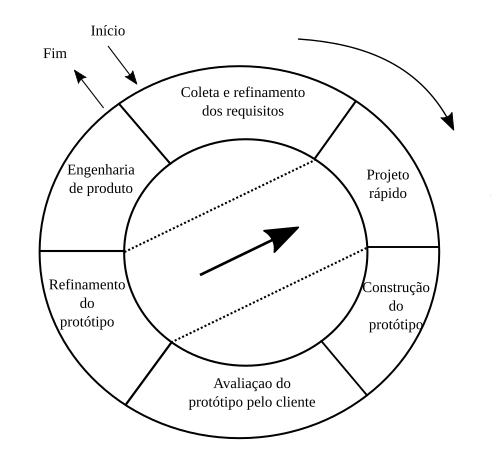
\includegraphics[width=0.45\textwidth,height=0.45\textheight,keepaspectratio]{figuras/prototipacao.png}
 \caption{Ciclo da prototipação \label{fig:prototipacao}}
 \vspace{-0.3cm}
 \caption*{Fonte: Adaptado de \cite[p.36]{pressman}.}
\end{figure}

%As etapas estão divididas da seguinte maneira:
\begin{enumerate}

 \item Definição dos componentes: %Com base na análise dos requisitos do sistema, xxxx em \citeonline{pressman}
Segundo \citeonline{pressman}, a primeira fase da engenharia de \textit{hardware} 
compreende a análise de requisitos de \textit{hardware} e o planejamento de desenvolvimento, o qual estabelece a finalidade dos 
dispositivos. Com base nisso, serão escolhidos os componentes que façam com que os objetivos de projeto possam ser executados;

 \item Condicionamento de sinais: São utilizados sensores para que grandezas físicas pertinentes possam ser aferidas pelo sistema, 
 tais como velocidade e tensão elétrica. No entanto, para que o dispositivo de aquisição de sinais possa medir 
 o valor dos sensores eficaz e corretamente, se faz necessário fazer o condicionamento de sinais destes dispositivos. Este 
 processo será feito através das descrições contidas nos \textit{datasheets} (folha de especificação) dos componentes e por 
 simulações em \textit{softwares} de circuitos elétricos.
 
 %Esses sensores, por sua vez, necessitam de condicionamento de sinal para que o dispositivo de aquisição de dados efetue a medição de
 %forma eficaz e exata. As principais tecnologias de condicionamento de sinal fornecem melhorias distintas tanto no que diz respeito 
 %ao desempenho quanto à exatidão de sistemas de aquisição de dados.
%é necessário um tratamento destes sinais para que estes possam ser lidos 
 %apropriadamente pelo processador. Desta forma, esta etapa do trabalho se preocupa com que os sinais dos sensores possam 
 
 \item Projeto do protótipo: Esta parte consiste em projetar o \textit{chassi} do robô (a sua estrutura física) com todos os componentes 
 necessários para o seu funcionamento. Será utilizado um \textit{software} 
 \sigla{EDA}{\textit{Electronic Design Automation}} para a criação da placa de circuito impresso 
 (\sigla{PCB}{\textit{Printed Circuit Board}}). Nesta etapa também serão feitos os códigos no microcontrolador, que é o dispositivo 
 de processamento do sistema.
 
 \item Projeto do controlador: Para o projeto do controlador PID, será utilizada a modelagem experimental 
 para obter um modelo matemático, visto que é mais simples do que a fenomenológica, conforme diz \citeonline{allan}. Para este 
 controlador serão utilizados \textit{softwares} matemáticos para a simulação do modelo obtido. Para o projeto do controlador 
 de Sistemas a Eventos Discretos, será utilizado o modelo de Moore, pois é de fácil implementação e é oportuno ao que se deseja 
 implementar. Será utilizado uma ferramenta	 computacional de controle supervisório para esta modelagem.
 
 \item Sistema de telemetria: O sistema de telemetria tem o intuito de informar um operador externo sobre as condições de operação do 
 robô. Neste trabalho, serão transmitidas informações como a velocidade do robô e o traçado da pista. A comunicação será feita por um 
 dispositivo \textit{bluetooth}.
 
 \item Integração do sistema e implementação do protótipo: Com as etapas anteriores finalizadas, é necessário integrá-las. 
 A integração será feita com os sensores e atuadores sendo soldados ou acoplados na PCB e os controladores e a aquisição de sinais 
 implementados no microcontrolador. 
 
 \item Testes de desempeho: Serão realizados testes de desempenho de modo a verificar o que pode ou o que precisa ser 
 melhorado no protótipo. Podem ser feitos ajustes tanto de \textit{hardware} 
 (como a substituição de componentes) quanto de \textit{software} (alterações no código do microcontrolador). Pode ser necessário 
 retornar a etapas anteriores para realizar estas correções.
 
 \item Implementação do projeto final: Com os testes de desempenho e as alterações necessárias feitas, é implementado o projeto final de 
 forma a validar este trabalho. Na versão final do veículo espera-se atingir os objetivos que foram propostos na Seção 
 \ref{objetivos}.
 
\end{enumerate}


%\noindent{\bf Definição de componentes:} 
%Segundo \citeonline{pressman}, a primeira fase da engenharia de \textit{hardware} 
%compreende a análise de requisitos de \textit{hardware} e o planejamento de desenvolvimento, o qual estabelece a finalidade dos 
%dispositivos. Com base nisso, serão escolhidos os componentes que façam com que os objetivos de projeto possam ser executados;








